\documentclass[%
%10pt,
%varwidth=false,
%crop=true,
border={0mm 0mm 0mm 0mm}]{standalone}
\usepackage[T1]{fontenc}
\usepackage[utf8]{inputenc}
\usepackage[auto]{microtype}
%\usepackage{cmbright}
\usepackage{arev}
\usepackage{amsmath, amssymb, amsfonts, icomma}
\usepackage[version=4]{mhchem}
\usepackage{tikz}
\usetikzlibrary{positioning, matrix}
\usepackage{chemplants-tub}
\usepackage{xcolor}
%define stream tip, default is stealth
\setchpstreamtip{latex}
\setchpmainstreamthickness{thick}
%\setchpunitthickness{very thick}

\pgfdeclarelayer{bg}    % declare background layer
\pgfsetlayers{bg,main}  % set the order of the layers (main is the standard layer)

\definecolor{signalgruen}{RGB}{49,127,67}    % RAL 6032 Wasser
\definecolor{signalrot}{RGB}{155,36,35}      % RAL 3001 Dampf
\definecolor{signalgrau}{RGB}{150,153,146}   % RAL 7004 Luft
\definecolor{signalgelb}{RGB}{229,190,001}   % RAL 1003 brennbare und nicht brennbare Gase
\definecolor{signalorange}{RGB}{208,93,40}   % RAL 2010 Säuren
\definecolor{signalviolett}{RGB}{132,76,130} % RAL 4008 Laugen
\definecolor{signalbraun}{RGB}{121,77,62}    % RAL 8002 brennbare und nicht brennbare Flüssigkeiten
\definecolor{signalblau}{RGB}{30,45,110}     % RAL 5005 Sauerstoff

% TABLEAU-10
\definecolor{Tab10-A}{RGB}{78, 121, 167}
\definecolor{Tab10-B}{RGB}{242, 142, 43}
\definecolor{Tab10-C}{RGB}{225, 87, 89}
\definecolor{Tab10-D}{RGB}{118, 183, 178}
\definecolor{Tab10-E}{RGB}{89, 161, 79}
\definecolor{Tab10-F}{RGB}{237, 201, 72}
\definecolor{Tab10-G}{RGB}{176, 122, 161}
\definecolor{Tab10-H}{RGB}{255, 157, 167}
\definecolor{Tab10-I}{RGB}{156, 117, 95}
\definecolor{Tab10-J}{RGB}{186, 176, 172}

\begin{document}
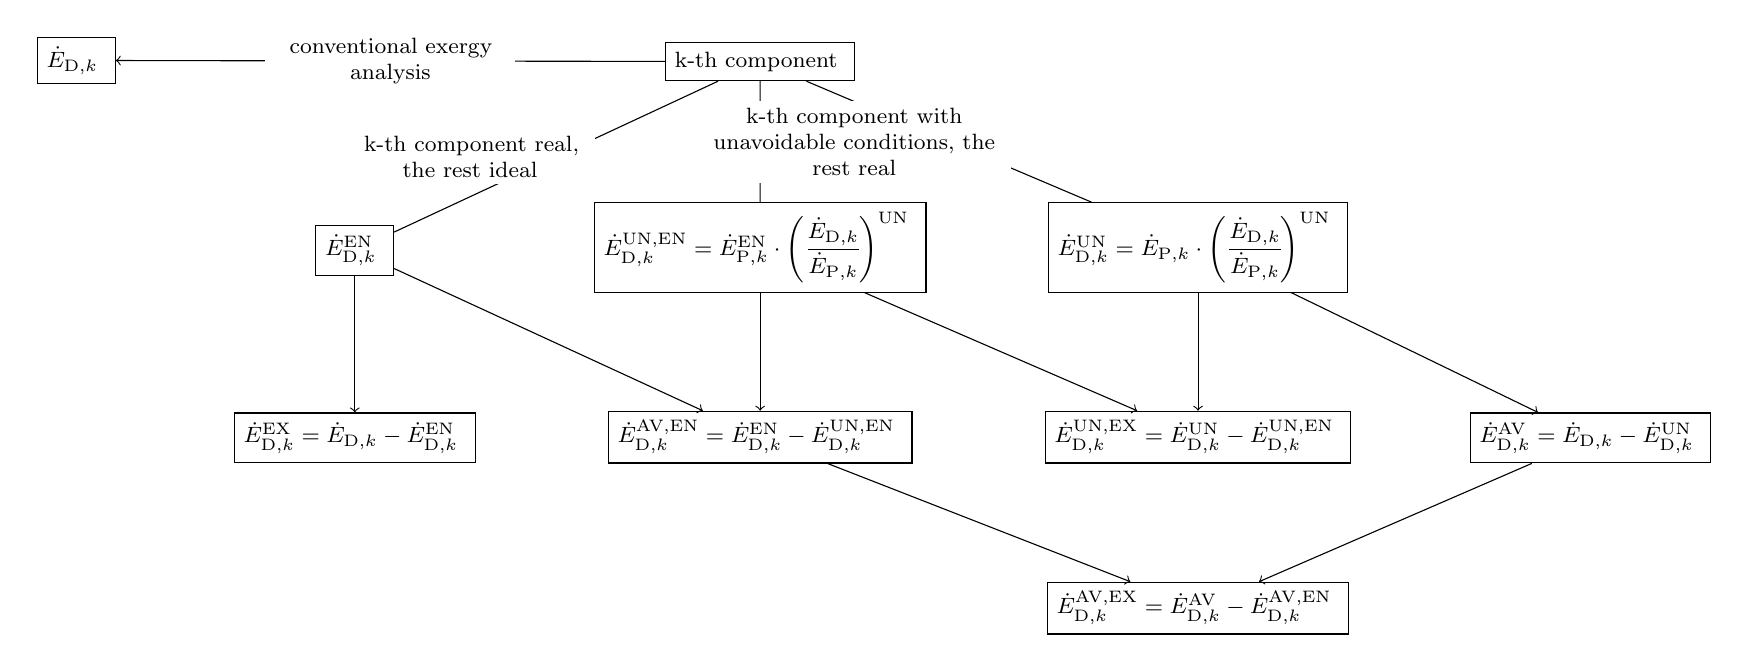
\begin{tikzpicture}[font=\footnotesize, node distance=15mm and 15mm]
  \pgfdeclarelayer{background}
  \pgfsetlayers{main,background}
  \matrix (m) [
    matrix of nodes,
    nodes={draw, align=center},
    column sep=15mm,
    row sep=15mm,
  ] {
    $\dot{E}_{\text{D},k}$ & & k-th component & & \\
    |[draw=none]| & $\dot{E}_{\text{D},k}^\text{EN}$ & $\dot{E}_{\text{D},k}^{\text{UN,EN}} = \dot{E}_{\text{P},k}^{\text{EN}} \cdot \left( \cfrac{\dot{E}_{\text{D},k}}{\dot{E}_{\text{P},k}} \right)^\text{UN}$ & $\dot{E}_{\text{D},k}^{\text{UN}} = \dot{E}_{\text{P},k} \cdot \left( \cfrac{\dot{E}_{\text{D},k}}{\dot{E}_{\text{P},k}} \right)^\text{UN}$ & \\
    |[draw=none]| & $\dot{E}_{\text{D},k}^{\text{EX}} = \dot{E}_{\text{D},k} - \dot{E}_{\text{D},k}^\text{EN}$ & $\dot{E}_{\text{D},k}^{\text{AV,EN}} = \dot{E}_{\text{D},k}^{\text{EN}} - \dot{E}_{\text{D},k}^{\text{UN,EN}} $ & $\dot{E}_{\text{D},k}^{\text{UN,EX}} = \dot{E}_{\text{D},k}^{\text{UN}} - \dot{E}_{\text{D},k}^{\text{UN,EN}}$ & $\dot{E}_{\text{D},k}^{\text{AV}} = \dot{E}_{\text{D},k} - \dot{E}_{\text{D},k}^{\text{UN}}$ \\
    |[draw=none]| & & & $\dot{E}_{\text{D},k}^{\text{AV,EX}} = \dot{E}_{\text{D},k}^{\text{AV}} - \dot{E}_{\text{D},k}^{\text{AV,EN}} $ & \\
  };

  \begin{scope}[
    font=\footnotesize,
    inner sep=.25em,
  ]
    \draw[->]
      (m-1-3) -- node[midway, left=-0.5cm, fill=white] {\parbox{3cm}{\centering k-th component real, the rest ideal}} (m-2-2)
      (m-1-3) -- node[midway, right=-0.8cm, fill=white] {\parbox{3.8cm}{\centering {k-th component with unavoidable conditions, the rest real}}}  (m-2-3)
      (m-1-3) -- node[midway, left] {} (m-2-4)
      (m-1-3) -- node[midway, fill=white] {\parbox{3cm}{\centering conventional exergy analysis}} (m-1-1);
    \draw[->]
      (m-2-2) -- (m-3-2);
    \draw[->]
      (m-2-2) -- (m-3-3);
    \draw[->]
      (m-2-3) -- (m-3-3);
    \draw[->]
      (m-2-3) -- (m-3-4);
    \draw[->]
      (m-2-4) -- (m-3-4);
    \draw[->]
      (m-2-4) -- (m-3-5);
    \draw[->]
      (m-3-3) -- (m-4-4);
    \draw[->]
      (m-3-5) -- (m-4-4);
  \end{scope}
\end{tikzpicture}
\end{document}

